\begin{frame}{What is the HHL algorithm?}

    \iconcite{Harrow_2009} \\
    Let $Ax = b$ a linear system, $A\in\mathbb{R}^{N_b \times N_b}, \mathbf{b} \in \mathbb{R}^{N_b}$
    \vspace{\baselineskip}
    \begin{itemize}
        \item \textbf{Input limitations:} $A$ sparse and hermitian
        \item \textbf{Output limitations:}
        \begin{itemize}
            \item HHL \textbf{does not} actually compute $x$ (\textit{amplitude encoding})
            \item HHL computes a \textit{feature} of $x$, e.g., $x^\top M x$ 
        \end{itemize}
        \item \textbf{Logarithmic scaling in $N_b$:} \\ 
        \begin{equation*}
            \mathcal{O}(\log N_b \kappa^2/\epsilon) \quad \text{vs} \quad \mathcal{O}(N_b \kappa)
        \end{equation*}
        $\kappa$: condition number of $A$, $\epsilon$: desired accuracy
    \end{itemize}
\end{frame}

\begin{frame}{Basic idea}
    Given the eigenvalue decomposition (EVD) of the matrix, $A = \sum_i \lambda_i\mathbf{u}_i\mathbf{u}_i^\top$, its inverse can be computed as
    \begin{equation*}
        A^{-1} = \sum_i \lambda_i^{-1}\mathbf{u}_i\mathbf{u}_i^\top
    \end{equation*}
    Thus, if we rewrite $\mathbf{b}$ in the eigenvector basis, $\mathbf{b} = \sum_i \beta_i \mathbf{u}_i$, $\mathbf{x}$ will be
    \begin{align*}
        \mathbf{x} 
        = A^{-1}\mathbf{b}
        = \sum_i \lambda_i^{-1}\mathbf{u}_i\mathbf{u}_i^\top \mathbf{b}
        = \sum_i \lambda_i^{-1} \beta_i \mathbf{u}_i
    \end{align*}
\end{frame}

\begin{frame}{HHL implementation}
    \only<1>{
        Registers:
        \begin{itemize}
        \item \textit{b-register}: components of $\mathbf{b}, \mathbf{x}$, (\textit{amplitude encoding}), $n_b$-qubits, with $N_b = 2^{n_b}$
        \item \textit{c-register}: phase of the eigenvalues of $A$
        \item \textit{ancilla}: inversion and measurement
    \end{itemize}
    }
    \only<2>{
        Initial state:
        \begin{equation*}
            \ket{\Psi_0} = \ket{0}^{\otimes n_b}\ket{0}^{\otimes n_c}\ket{0}
        \end{equation*}   
    }
    \only<3>{
        Steps:
        \begin{multicols}{2}
        \begin{enumerate}
            \item State preparation
            \item QPE
            \item Ancilla qubit rotation
            \item Inverse QPE
        \end{enumerate}
        \end{multicols}
    }
    \begin{center}
    \begin{quantikz}
        % Ancilla qubit (single wire)
        \lstick{anc} &
            &
            &
            &
            \gate[style={fill=orange!20}]{R_y} &
            &
            \meter{} \rstick{$\ket{1}$?} \\

        % Clock register (multi-qubit bundle)
        \lstick{c-reg} &
            \qwbundle{n_c} &
            &
            \gate[2,style={fill=blue!10}]{\text{QPE}(e^{iAt})} &
            \ctrl{-1} &
            \gate[2,style={fill=blue!10}]{\text{QPE}^{\dagger}(e^{-iAt})} &
            \rstick{$\ket{0}$} \\

        % Input/Output register (multi-qubit bundle)
        \lstick{b-reg} &
            \qwbundle{n_b} &
            \gate[style={fill=green!20}]{\mathbf{b}\text{-enc}} &
            &
            &
            &
            \rstick{$\ket{x}$}
    \end{quantikz}
    \end{center}
\end{frame}

\begin{frame}{State preparation}
    \textbf{State preparation:} rotate the qubits in the b-register to have amplitudes corresponding to the coefficients of $\mathbf{b}$ (\textit{amplitude encoding})

    \vspace{\baselineskip}
    An example: $\mathbf{b} = (0,1), N_b = 2 \implies n_b = 1$

    \begin{center}
    \begin{quantikz}
        % Input/Output register (multi-qubit bundle)
        \lstick{b-reg} &
            \qwbundle{1} &
            \gate[style={fill=green!20}]{X} &
            \rstick{$\ket{1}$}
    \end{quantikz}
    \end{center}

    \vspace{\baselineskip}
    Recall:
    \begin{itemize}
        \item state preparation step specific to each $\mathbf{b}$ 
        \item $\mathbf{b}$ needs to be normalized: $\sum_i |\tilde{b}_i|^2 = 1$
        \item output: $\ket{\Psi_0} = \ket{\mathbf{b}}\ket{0}^{\otimes n_c}\ket{0}$
    \end{itemize}
\end{frame}

\begin{frame}{Quantum Phase Estimatation (QPE)}
    \textbf{Goal:} estimate the phase of the eigenvalues of $A$ \\
    \vspace{\baselineskip}
    Issues:
    \begin{itemize}
        \item How to encode matrix $A$ in the circuit? \textit{Hamiltonian encoding}
        \item How to estimate its eigenvalues? \textit{Quantum Phase Estimation}
    \end{itemize}
\end{frame}

\begin{frame}{Hamiltonian encoding}
    In general, $A$ non-unitary: we'll use
    \begin{equation*}
        U = e^{iAt}
    \end{equation*}
    which is unitary and can be approximated by solving a \textit{Hamiltonian simulation} problem
    
    \begin{center}
    \begin{quantikz}&
            \qwbundle{n_b} &
            \gate[style={fill=green!20}]{e^{iAt}} &
    \end{quantikz}
    \end{center}

    \begin{problem}[Hamiltonian Simulation Problem]
        Given a  Hamiltonian ($2^{n_b}\times 2^{n_b}$ Hermitian matrix), $A$, a time $t$ and a tolerance $\epsilon$, find $U$ such that 
        \begin{equation*}
            ||U-e^{iAt}|| \leq \epsilon
        \end{equation*}
    \end{problem}
    Algorithm: Trotterization + Pauli gadget ($A = \sum_j A_j$, $U \approx \prod_j e^{iA_jt}$)
\end{frame}

\begin{frame}{Quantum Phase Estimation (QPE)}
    Eigenvalue connection: $\text{eig}(U) = e^{i\lambda_j t}$, where $\lambda_j$ eigenvalues of $A$ \\

    \begin{center}
    \begin{quantikz}
        % Clock register (multi-qubit bundle)
        \lstick{$\ket{0}_{c_0}$} &
            \qwbundle{1} &
            \gate[style={fill=blue!10}]{H} &
            &
            \ctrl{2} &
            \gate[2,style={fill=blue!10}]{\text{IQFT}} &
            \rstick[3]{$\sum_j \beta_j \ket{u_j}_b \ket{\lambda_j}_c$} \\
        
        \lstick{$\ket{0}_{c_1}$} &
            \qwbundle{1} &
            \gate[style={fill=blue!10}]{H} &
            \ctrl{1} &
            &
            & \\

        % Input/Output register (multi-qubit bundle)
        \lstick{$\ket{b}$} &
            \qwbundle{n_b} &
            &
            \gate[style={fill=blue!10}]{U^{2^0}} &
            \gate[style={fill=blue!10}]{U^{2^1}}&
            &
            
    \end{quantikz}
    \end{center}
    

    Steps:
    \begin{enumerate}
        \item Superposition
        \item Controlled rotations
        \item Inverse Quantum Fourier Transforms (IQFT)
    \end{enumerate}
\end{frame}

\begin{frame}[allowframebreaks]{QPE: Controlled Rotations}

    After the superposition:
    \begin{equation*}
        \ket{\Psi_2} = \ket{b} \frac{1}{2^{\frac{n_c}{2}}} (\ket{0}+\ket{1})^{\otimes n} \ket{0}
    \end{equation*}

    \vspace{\baselineskip}

    For the moment, let's assume $\ket{b}$ eigenvector of $U$ with eigenvalue $e^{2\pi i \phi}$ (we can always express $\ket{b} = \sum_j \beta_j \ket{u_j}$), then:
    \begin{equation*}
        U \ket{b} = e^{2\pi i \phi} \ket{b}
    \end{equation*}

    \framebreak
    
    If the control is $0$, $\ket{b}$ is not affected, otherwise $U$ is applied. This is equivalent to (\textit{phase kickback}):
    %TODO: add U\ket{b} for clarity
    \begin{align*}
        \ket{\Psi_3} &= \ket{b} \otimes (\frac{1}{2^{\frac{n_c}{2}}} (\ket{0}+e^{2\pi i \phi 2^{n_c-1}}\ket{1}) \otimes \cdots \otimes (\ket{0}+e^{2\pi i \phi 2^{0}}\ket{1})) \otimes \ket{0}_a \\
        &= \ket{b} \otimes (\frac{1}{2^{\frac{n_c}{2}}}\bigotimes_{j=1}^{n_c}(\ket{0}+e^{2\pi i \phi 2^{n_c-j}}\ket{1})) \otimes \ket{0}_a \\
        &= \ket{b} \otimes (\frac{1}{2^{\frac{n_c}{2}}}\sum_{k=1}^{2^{n_c}-1} e^{2\pi i \phi k} \ket{k}) \otimes \ket{0}_a 
    \end{align*}
    \textbf{Motivation:} transfer phase information from $U$ to the control-qubits (\textit{c-registers})!
\end{frame}

% TODO: maybe add general purpose of IQFT
\begin{frame}{QPE: Inverse Fourier Transform}
    
\end{frame}


\begin{frame}{QPE: Inverse Fourier Transform}
    To extract the phase information from the \textit{c-registers} of $\ket{\Psi_3}$, IQFT is applied:
    \begin{align*}
        \mathrm{IQFT}(\frac{1}{2^{\frac{n_c}{2}}}\sum_{k=0}^{2^{n_c-1}}(e^{2\pi i \phi k}\ket{k})) &=  \frac{1}{2^{\frac{n_c}{2}}}\sum_{k=0}^{2^{n_c-1}}(e^{2\pi i \phi k}\mathrm{IQFT}(\ket{k})) \\
        &= \frac{1}{2^{\frac{n_c}{2}}}\sum_{k=0}^{2^{n_c-1}}(e^{2\pi i \psi k}(\frac{1}{\sqrt{2^{n_c}}}\sum_{j=0}^{N_c-1}e^{ -2\pi ijk/N_c}\ket{j})) \\
        &= \frac{1}{2^{n_c}}\sum_{k=0}^{2^{n_c-1}}(\sum_{j=0}^{2^{n_c}-1}e^{2\pi ik(\phi - j/N_c)}\ket{j})
    \end{align*}
\end{frame}

\begin{frame}{QPE: Inverse Quantum Fourier Transforms}
    
    Given the state before measurement: 
    $$\frac{1}{2^{n_c}} \sum_{k=0}^{2^{n_c}-1} \left( \sum_{j=0}^{2^{n_c}-1} e^{2\pi i k(\phi - j/N_c)} \ket{j} \right)$$
    
    The following alternatives apply:
    \vspace{0.2cm}
    \begin{itemize}
        \item \textbf{Constructive} (if $\phi - j/N_c = 0$): Amplitude proportional to $\sum e^0 = 2^{n_c}$
        \item \textbf{Destructive} (otherwise): Amplitude cancels since $\sum e^{2\pi i k(\dots)} = 0$
    \end{itemize}  
    
    
    \begin{figure}[htpb]
        \centering
        \begin{tikzpicture}[>=Stealth, scale=0.9, every node/.style={scale=0.85}]
            % ==========================================
            % 1. CONSTRUCTIVE: ORIGIN (Far Left)
            % ==========================================
            \begin{scope}[xshift=-4.5cm]
                \draw[->, gray!70, dashed] (-0.2,0) -- (1.5,0) node[right, font=\tiny] {Re};
                \draw[->, gray!70, dashed] (0,-1.0) -- (0,1.0) node[above, font=\tiny] {Im};
                \draw[->, ultra thick, blue] (0,0) -- (1.2, 0) node[midway, above=2pt, font=\tiny, align=center] {Overlapped\\phasors};
            \end{scope}
            
            % ==========================================
            % 2. CONSTRUCTIVE: TIP-TO-TAIL (Center Left)
            % ==========================================
            \begin{scope}[xshift=-2cm]
                \draw[->, gray!70, dashed] (-0.2,0) -- (2.6,0) node[right, font=\tiny] {Re};
                \draw[->, gray!70, dashed] (0,-1.0) -- (0,1.0) node[above, font=\tiny] {Im};
                
                \coordinate (curr) at (0,0);
                \foreach \k in {1,...,8} {
                    \draw[->, thick, blue] (curr) -- ++(0:0.25) coordinate (curr);
                    \draw[blue, thin] (curr) ++(0,0.05) -- ++(0,-0.1);
                }
                \draw[decoration={brace, amplitude=3pt, raise=4pt}, decorate, thick] 
                    (0,0) -- (curr) node[midway, above=6pt, font=\tiny] {Sum $= 2^{n_c}$};
            \end{scope}

            % ==========================================
            % VERTICAL DIVIDER (Center)
            % ==========================================
            \draw[thick, gray!30] (0, 1.2) -- (0, -1.2);

            % ==========================================
            % 3. DESTRUCTIVE: ORIGIN (Center Right)
            % ==========================================
            \begin{scope}[xshift=2cm]
                \draw[->, gray!70, dashed] (-1.2,0) -- (1.2,0) node[right, font=\tiny] {Re};
                \draw[->, gray!70, dashed] (0,-1.0) -- (0,1.0) node[above, font=\tiny] {Im};
                \foreach \k in {0,...,7} {
                    \draw[->, thick, red] (0,0) -- (\k*45:0.9);
                }
            \end{scope}

            % ==========================================
            % 4. DESTRUCTIVE: TIP-TO-TAIL (Far Right)
            % ==========================================
            \begin{scope}[xshift=4.5cm]
                \draw[->, gray!70, dashed] (-0.5,0) -- (1.5,0) node[right, font=\tiny] {Re};
                \draw[->, gray!70, dashed] (0,-0.5) -- (0,1.5) node[above, font=\tiny] {Im};

                \coordinate (curr2) at (0,0);
                \foreach \k in {0,...,7} {
                    \draw[->, thick, red] (curr2) -- ++(\k*45:0.35) coordinate (curr2);
                }
                \filldraw[black] (0,0) circle (1.5pt) node[below left=1pt, font=\tiny\bfseries] {Sum $= 0$};
            \end{scope}
        \end{tikzpicture}
    \end{figure}
\end{frame}

% TODO: add a comment on the selection of t,n_c
\begin{frame}{QPE: Inverse Quantum Fourier Transforms}
    Finally, ignoring the states with zero-amplitude:
    \begin{align*}
        \ket{\Psi_4} &= \frac{1}{2^n}\ket{b}\sum_{k=0}^{2^n-1} e^{2\pi ik \cdot 0} \ket{N_c\phi}\ket{0}_a \\
        &= \ket{b}\ket{N_c\phi}\ket{0}_a
    \end{align*}
    The \textit{c-registers} qubits are used to represent the phase information of $U$!
\end{frame}

\begin{frame}{QPE: Inverse Quantum Fourier Tranform}
    Recap:
    \begin{itemize}
        \item We assumed: $\ket{b}$ eigenvector of $U$ with eigenvalue $e^{2\pi i \phi}$
        \item $U$ encodes $A$ as $U = e^{iAt}$, so that $U\ket{b} = e^{i\lambda_j t} \ket{b}$
    \end{itemize}

    \vspace{0.2cm}
    Thus, $ \phi = \frac{\lambda_j t}{2\pi}$ and
    \begin{equation*}
        \ket{\Psi_4} = \ket{u_j}\ket{\frac{N_c \lambda_j t}{2\pi}}\ket{0}_a
    \end{equation*}
\end{frame}

\begin{frame}{QPE: Inverse Fourier Transform V}
    More generally, writing $\ket{b} = \sum_j \beta_j \ket{u_j}$ 
    \begin{equation*}
        \ket{\Psi_4} = \sum_{j=0}^{2^{n_b}-1} b_j\ket{u_j} \ket{\frac{N_c\lambda_j t}{2\pi}}\ket{0}_a
    \end{equation*} 
    % TODO: check the statement about the params
    \textbf{Note:} $\ket{\frac{N_c\lambda_j t}{2\pi}}$ encoded through basis-encoding. $t, N_c$ to make the latter integers
\end{frame}


\begin{frame}{Ancilla qubit}
    Rotation of the ancilla qubit: eigenvalue inversion, depends on a parameter $C$
    \begin{equation*}
        \ket{\Psi_5} = \sum_{j=0}^{2^{n_b}-1} b_j\ket{u_j}\ket{\tilde{\lambda_j}}(\sqrt{1-\frac{C^2}{\tilde{\lambda}_j^2}}\ket{0}_a + \frac{C}{\tilde{\lambda}_j}\ket{1}_a)
    \end{equation*}

\end{frame}
\begin{frame}{Ancilla qubit}

    \begin{columns}
    \begin{column}{0.5\textwidth}
        Ry-gates: 
        \begin{align*}
            R_y(\theta_j) =
            \begin{bmatrix}
                \cos(\theta_j/2) & -\sin(\theta_j/2) \\
                \sin(\theta_j/2) & \cos(\theta_j/2)
            \end{bmatrix} 
        \end{align*}
        and angle 
        \begin{equation*}
            \theta_j = \arcsin(\frac{C}{\lambda_j})
        \end{equation*}
    \end{column}
    \begin{column}{0.5\textwidth}
        \begin{center}
        \begin{tikzpicture}[
            scale=1.8,
            vector/.style={thick,-{Stealth[length=2.5mm]}},
            axis/.style={thin,gray,-{Stealth}}
        ]
            % 1. Draw the 2D Bloch circle
            \draw[thick] (0,0) circle (1);

            % 2. Draw and label the X and Z axes
            \draw[axis] (-1.2,0) -- (1.2,0) node[right,black] {$x \; \ket{+}$};
            \draw[axis] (0,-1.2) -- (0,1.2) node[above,black] {$z \; \ket{0}$};
            \node[below,black] at (0,-1.05) {$\ket{1}$};
            \node[left,black] at (-1.05,0) {$\ket{-}$};

            % 3. Define the angles 
            % Note: In the Bloch sphere, the polar angle is measured from the Z-axis (Up).
            % In standard TikZ polar coordinates, angle 0 is the X-axis (Right) and 90 is the Z-axis.
            \def\gammatemp{0} % Initial state angle from Z
            \def\thetatemp{25} % Ry rotation angle

            % Convert Bloch angles to TikZ polar coordinates
            \pgfmathsetmacro\tikzgamma{90-\gammatemp}
            \pgfmathsetmacro\tikztotal{90-(\gammatemp+\thetatemp)}

            % 4. Draw the state vectors
            % Initial State
            \draw[vector, blue] (0,0) -- (\tikzgamma:1) 
                node[midway, above left=-2pt, inner sep=2pt] {$\ket{\psi}$};
                
            % Final State after Ry(theta)
            \draw[vector, red] (0,0) -- (\tikztotal:1) 
                node[midway, below right=-2pt, inner sep=2pt] {$Ry(\theta)|\ket{\psi}$};

            % 5. Draw the arcs to indicate the angles
        % Theta arc (from initial state to final state)
            \draw[-{Stealth}, thick, red] (\tikzgamma:0.5) arc (\tikzgamma:\tikztotal:0.5) 
                node[midway, right=1pt, inner sep=2pt] {};
            
            % 6. Add a center origin dot
            \filldraw[black] (0,0) circle (0.5pt);

        \end{tikzpicture}
        \end{center}
    \end{column}
    
    \end{columns}

    % TODO: circuit to implement rotation 

\end{frame}
\begin{frame}{Ancilla qubit}

    Once the ancilla qubit is measured we got two alternatives
    \begin{itemize}
        \item if $\ket{0}$: throw away the results
        \item if $\ket{1}$: store the results
    \end{itemize}
    \vspace{\baselineskip}
    After that the state is updated to 
    \begin{equation*}
        \ket{\Psi_6} = \frac{1}{\sum_{j=0}^{2^{n_b}-1} |\frac{b_j N_c}{\tilde{\lambda}_j}|^2}\sum_{j=0}^{2^{n_b}-1} b_j\ket{u_j}\ket{\tilde{\lambda_j}}\frac{C}{\tilde{\lambda}_j}\ket{1}_a
    \end{equation*}
\end{frame}

\begin{frame}{Inverse QPE I}
    \begin{equation*}
        \ket{\Psi_6} = \frac{1}{\sum_{j=0}^{2^{n_b}-1} |\frac{b_j N_c}{\tilde{\lambda}_j}|^2}\sum_{j=0}^{2^{n_b}-1} C\frac{b_j}{\tilde{\lambda}_j}\ket{u_j}\ket{\tilde{\lambda_j}}\ket{1}_a
    \end{equation*}

    Issues:
    \begin{itemize}
        \item b-registers are not encoded with respect to the canonical basis
        \item b-registers and c-registers are entagled
    \end{itemize}
\end{frame}

\begin{frame}{Inverse QPE: Quantum Fourier Transform}
    To do so, QFT is applied to the \textit{c-register} qubits:

    \begin{equation*}
        \mathrm{QFT}(\ket{\tilde{\lambda_j}}) = \frac{1}{2^{\frac{n}{2}}}\sum_{y=0}^{2^n-1} e^{2\pi iy\tilde{\lambda}_j/N_c}\ket{y}
    \end{equation*}
    leading to 
    \begin{align*}
        \ket{\Psi_7} = \frac{1}{\sum_{j=0}^{2^{n_b}-1} |\frac{b_j N_c}{\tilde{\lambda}_j}|^2} \sum_{j=0}^{2^{n_b}-1} C\frac{b_j}{\tilde{\lambda}_j}\ket{u_j}(\frac{1}{2^{\frac{n}{2}}}\sum_{y=0}^{2^n-1} e^{2\pi iy\tilde{\lambda}_j/N_c}\ket{y})\ket{1}_a
    \end{align*}
\end{frame}

\begin{frame}{Inverse QPE: Controlled rotations}
    Then controlled rotations with $U^{-1}$ are applied as before

    \begin{align*}
        &\sum_{j=0}^{2^{n_b}-1} C\frac{b_j}{\tilde{\lambda}_j}\ket{u_j}(\frac{1}{2^{\frac{n}{2}}}\sum_{y=0}^{2^n-1} e^{-i\lambda_j ty}e^{2\pi iy\tilde{\lambda}_j/N_c}\ket{y}) \\
        &= \sum_{j=0}^{2^{n_b}-1} C\frac{b_j}{\tilde{\lambda}_j}\ket{u_j}\sum_{y=0}^{2^n-1} \ket{y} 
        = C\ket{x}\sum_{y=0}^{2^n-1} \frac{1}{2^{\frac{n}{2}}}\ket{y}
    \end{align*}

    leading to 

    \begin{align*}
        \ket{\Psi_8} = \frac{C}{2^{\frac{n}{2}}\sum_{j=0}^{2^{n_b}-1} |\frac{b_j N_c}{\tilde{\lambda}_j}|^2} \ket{x}\sum_{y=0}^{2^n-1} \frac{1}{2^{\frac{n}{2}}}\ket{y}\ket{1}_a
    \end{align*}
\end{frame}

\begin{frame}{Inverse QPE IV}
    The clock-qubits and \textit{b-registers} are now unentagled. By applying the Hadamard gates to the clock qubits we have
    \begin{align*}
        \ket{\Psi_9} &= \frac{C}{\sum_{j=0}^{2^{n_b}-1} |\frac{b_j N_c}{\tilde{\lambda}_j}|^2} \ket{x}_b \ket{0}_c^{\otimes n}\ket{1}_a
    \end{align*}
    where the solution $\ket{x}$ is stored in the \textit{b-registers} successfully.
\end{frame}

\begin{frame}{Simulations}
    Linear system, $Ax = b$
    \begin{equation*}
        A = 
        \begin{bmatrix}
            1 & -1/3 \\
            -1/3 & 1    
        \end{bmatrix}, 
        \quad 
        b = \begin{bmatrix}
            0 \\
            1
        \end{bmatrix} 
    \end{equation*}

    Actual solution
    \begin{equation*}
        x = \begin{bmatrix}
            1.125 \\
            0.375
        \end{bmatrix}
    \end{equation*}
\end{frame}

\begin{frame}{Simulations: Quantum Emulator}
    \begin{figure}
        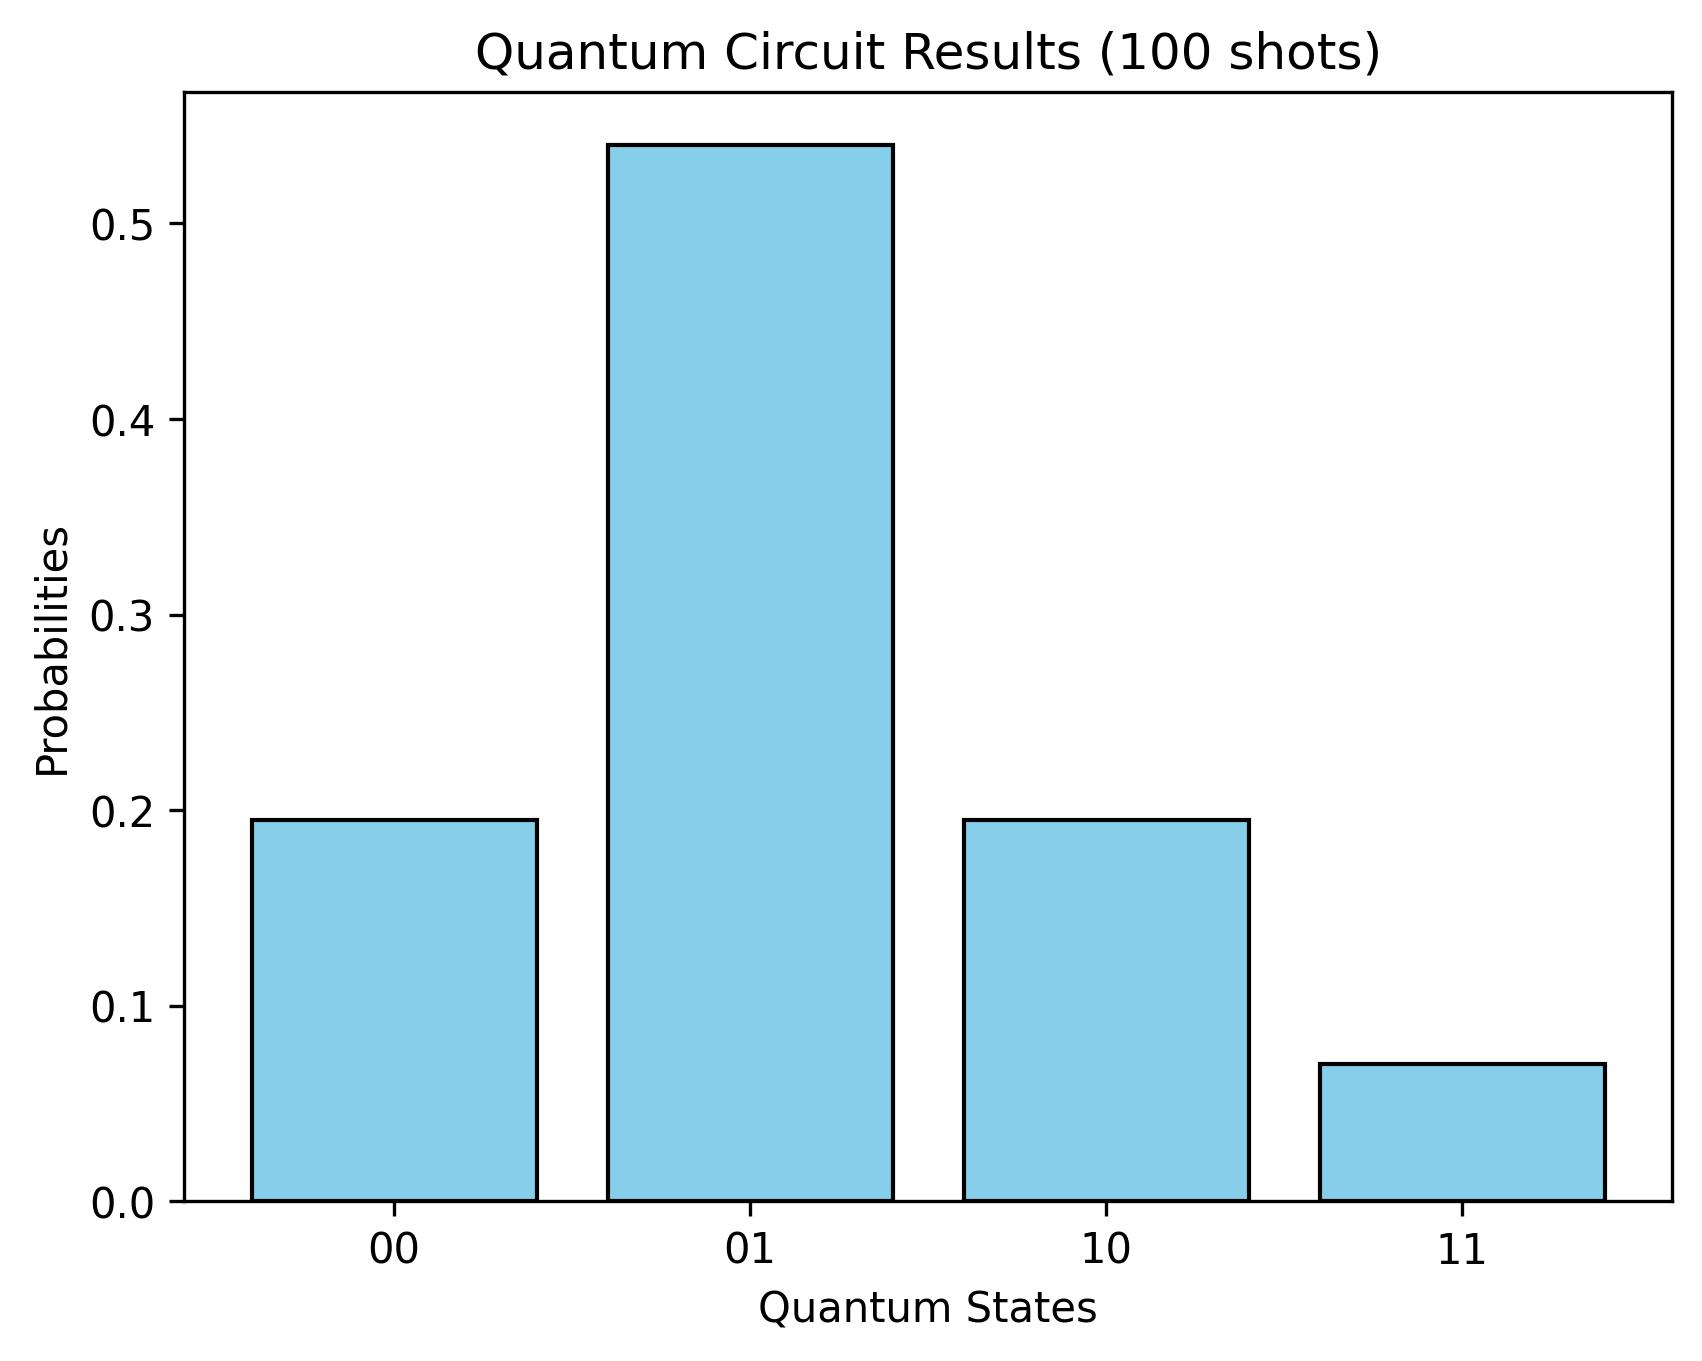
\includegraphics[width=0.75\textwidth]{plots/emulator-raw-measurements.jpeg}
    \end{figure}
\end{frame}

\begin{frame}{Simulations: Quantum Emulator}
    \begin{figure}
        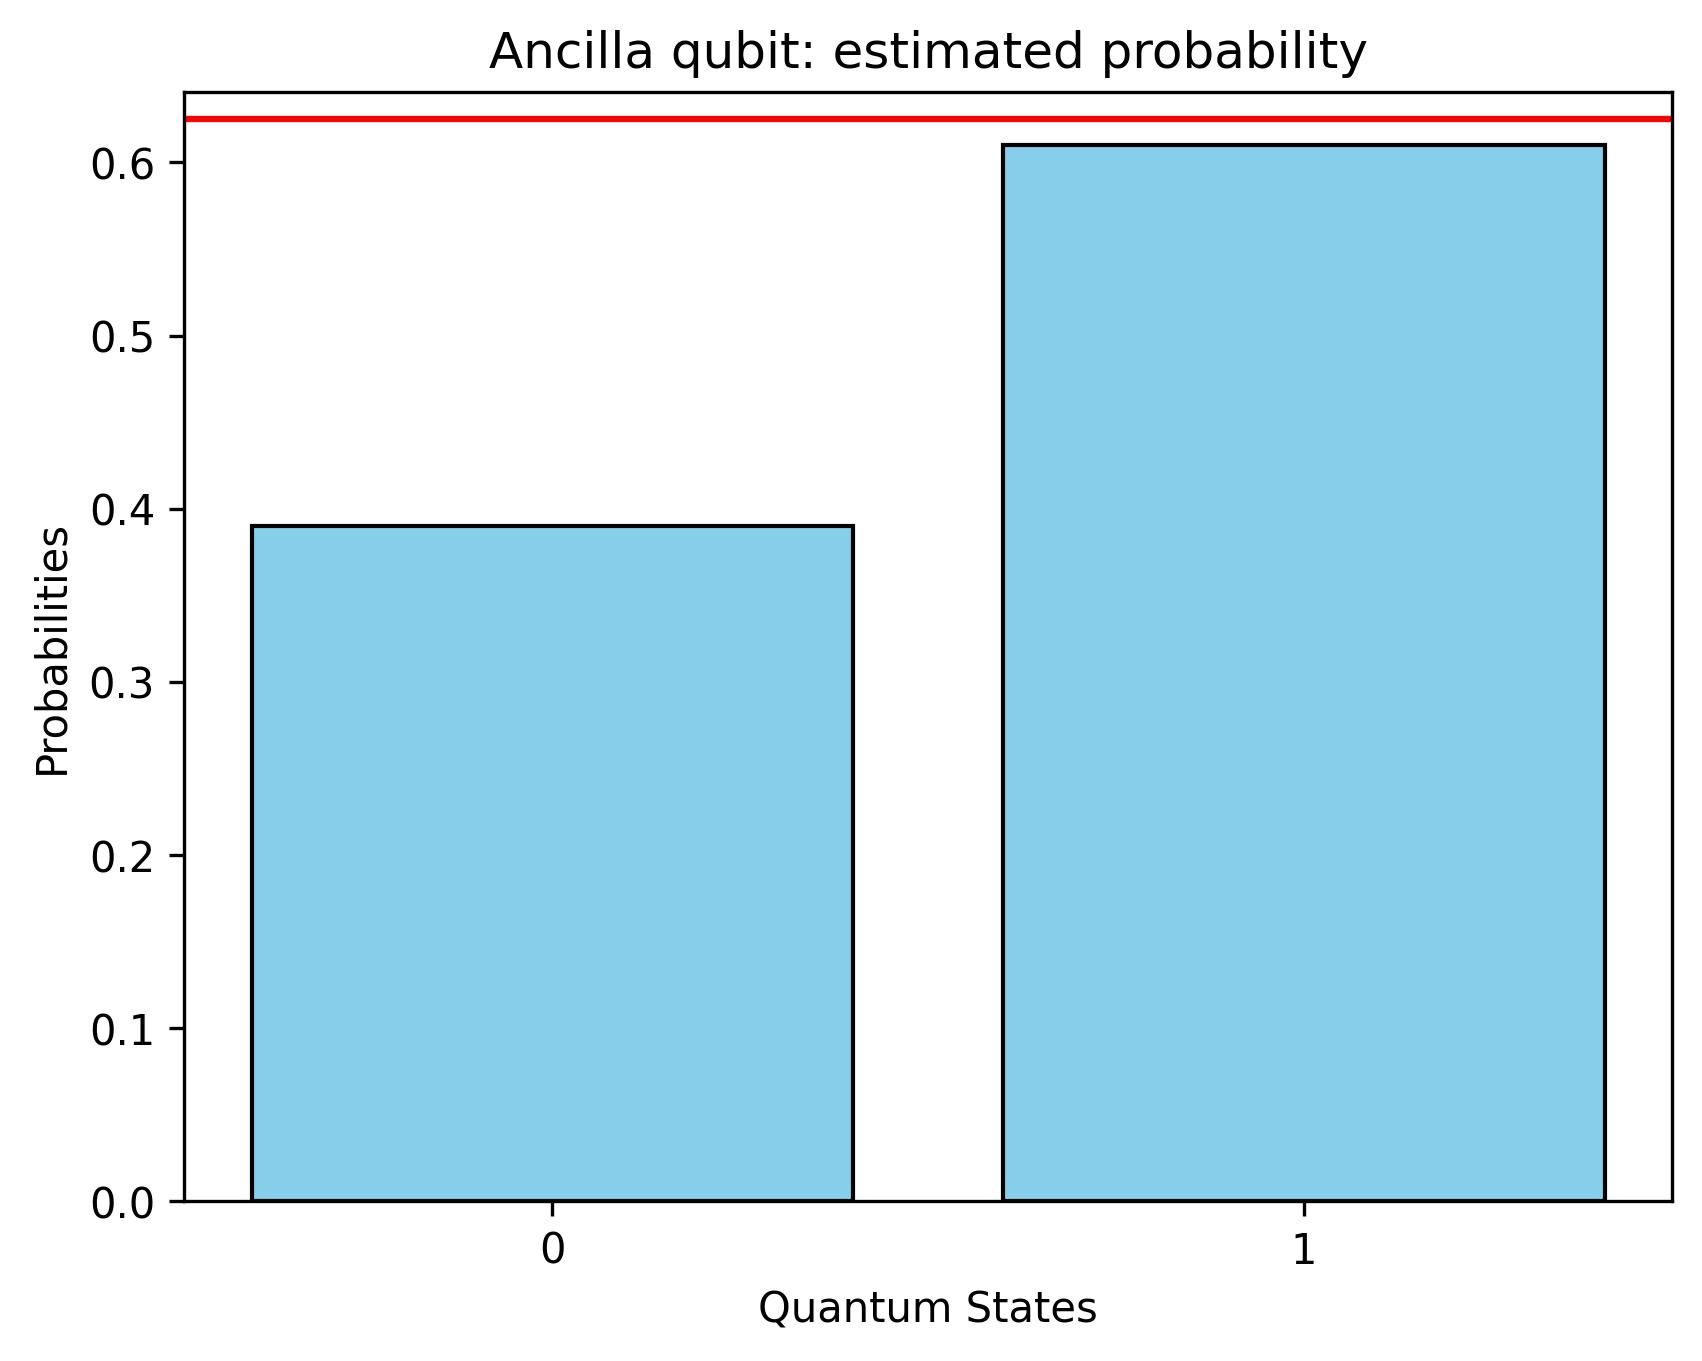
\includegraphics[width=0.75\textwidth]{plots/emulator-prob-anc.jpeg}
    \end{figure}
\end{frame}

\begin{frame}{Simulations: Quantum Emulator}
    \begin{figure}
        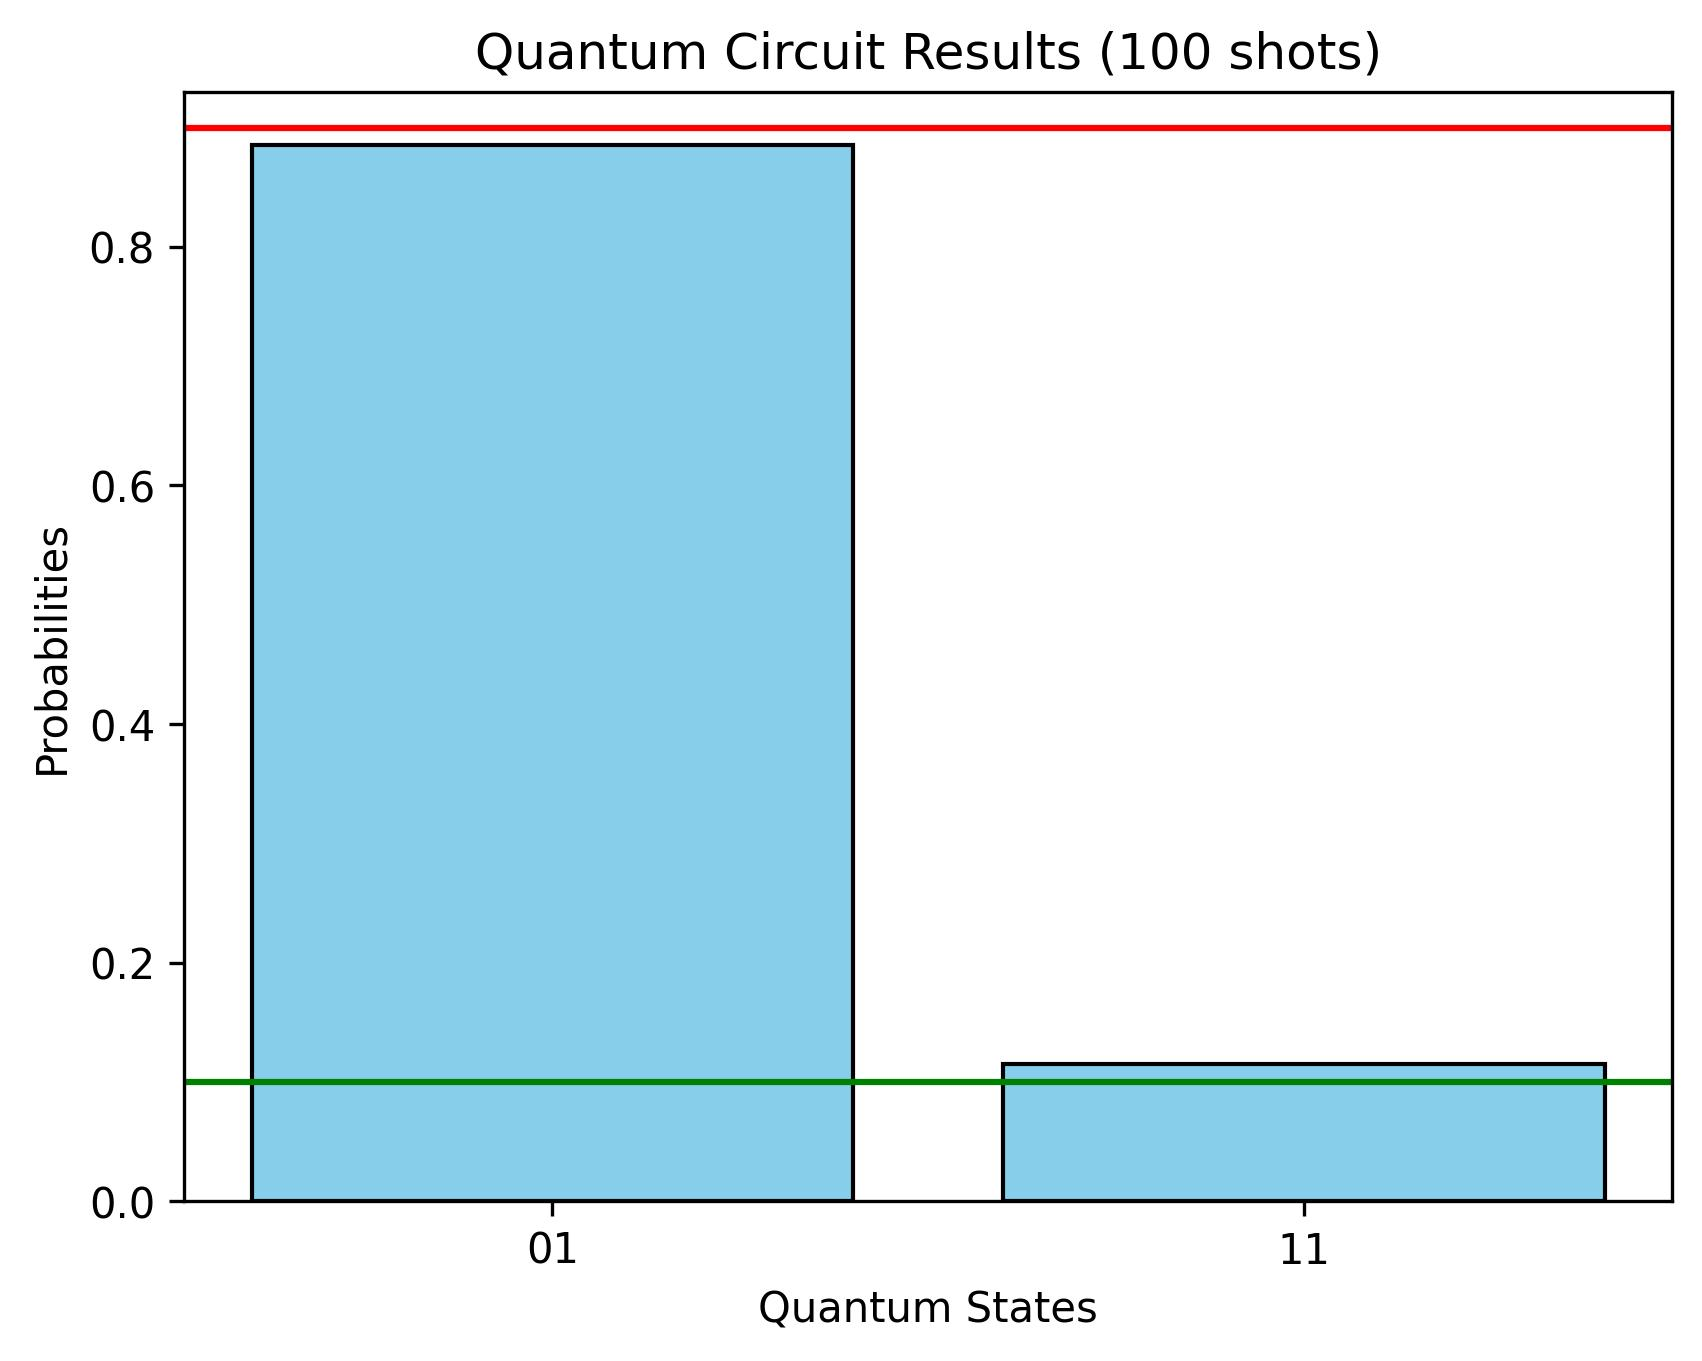
\includegraphics[width=0.75\textwidth]{plots/emulator-conditional-anc1.jpeg}
    \end{figure}
\end{frame}

\begin{frame}{Simulations: IBM Quantum Hardware}
     \begin{figure}
        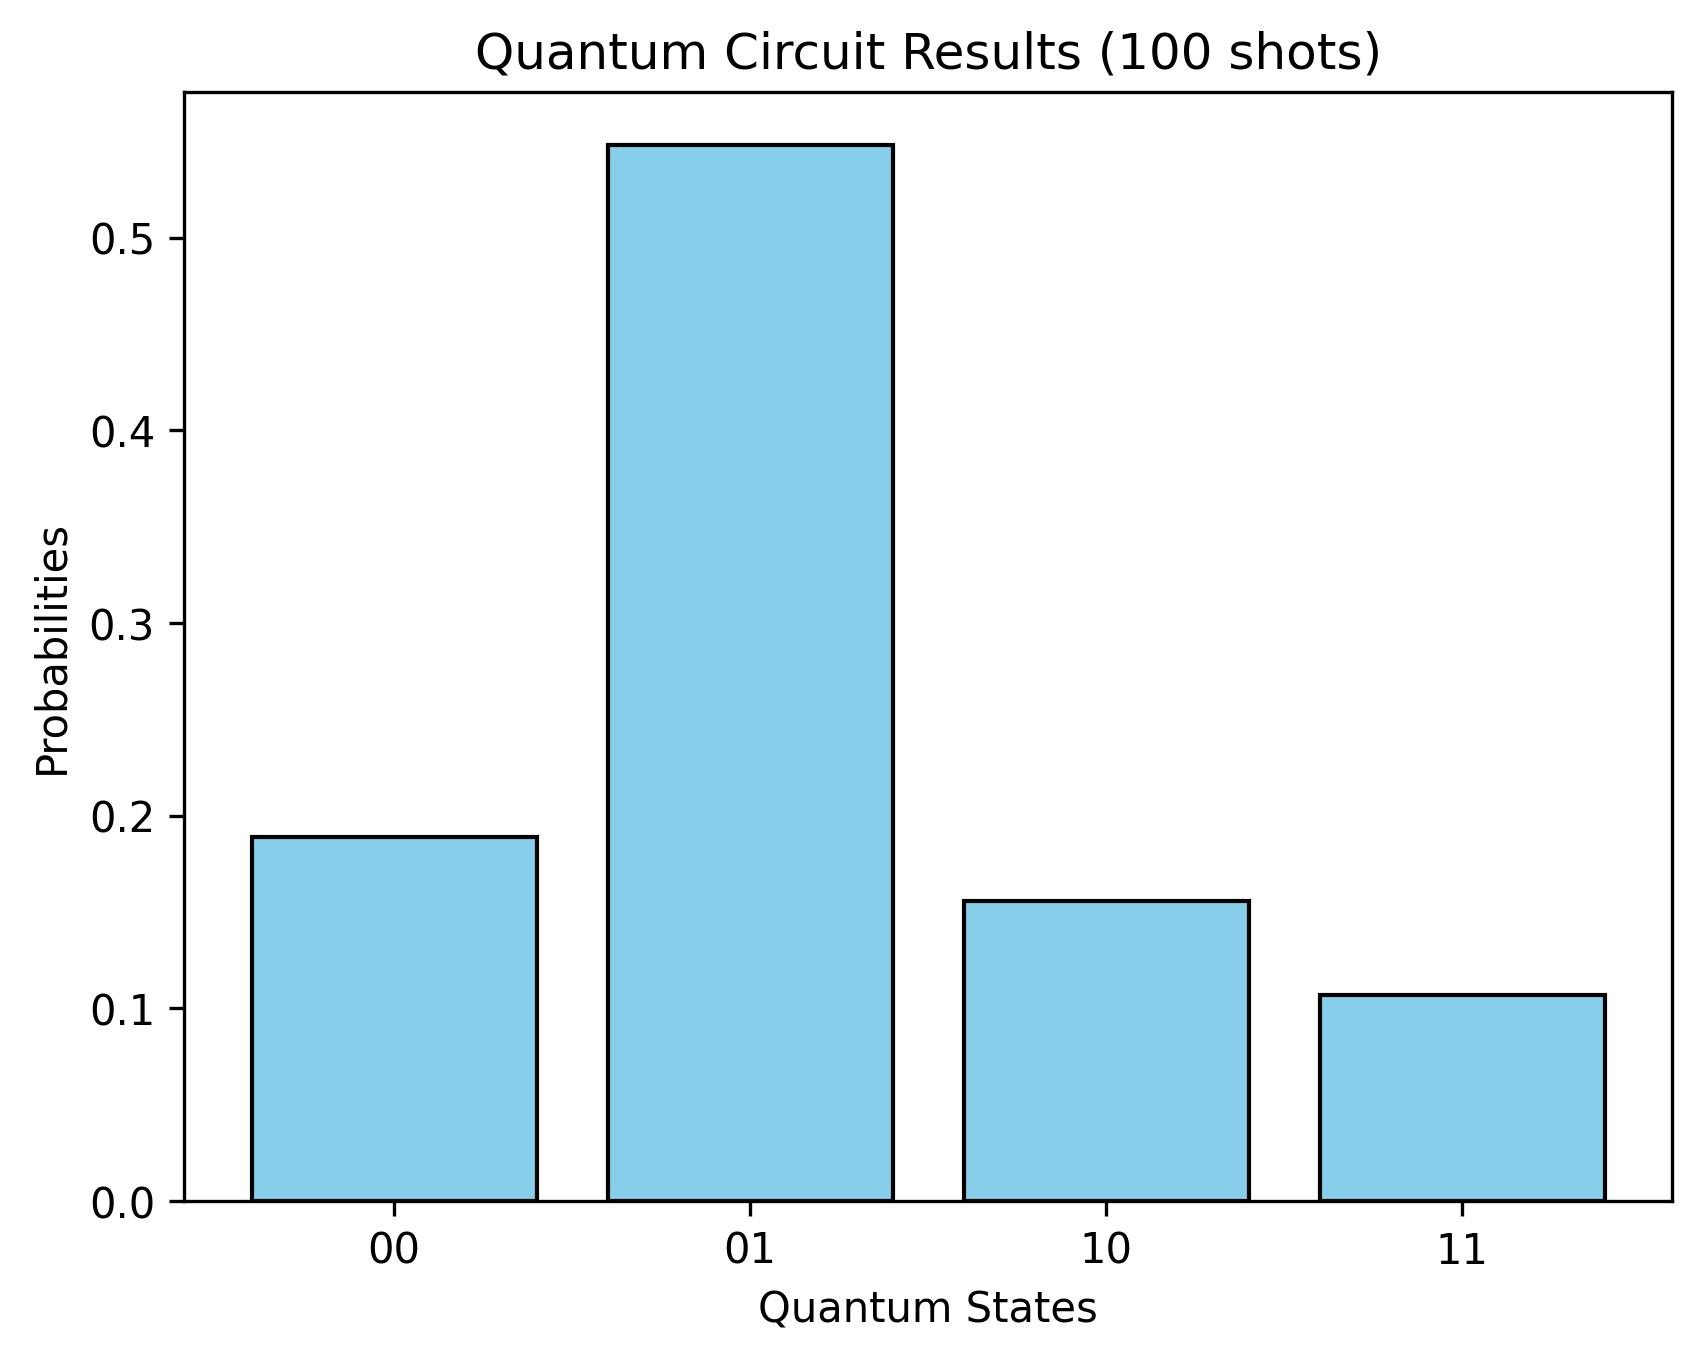
\includegraphics[width=0.75\textwidth]{plots/ibm-raw-measurements.jpeg}
    \end{figure}
\end{frame}

\begin{frame}{Simulations: IBM Quantum Hardware}
     \begin{figure}
        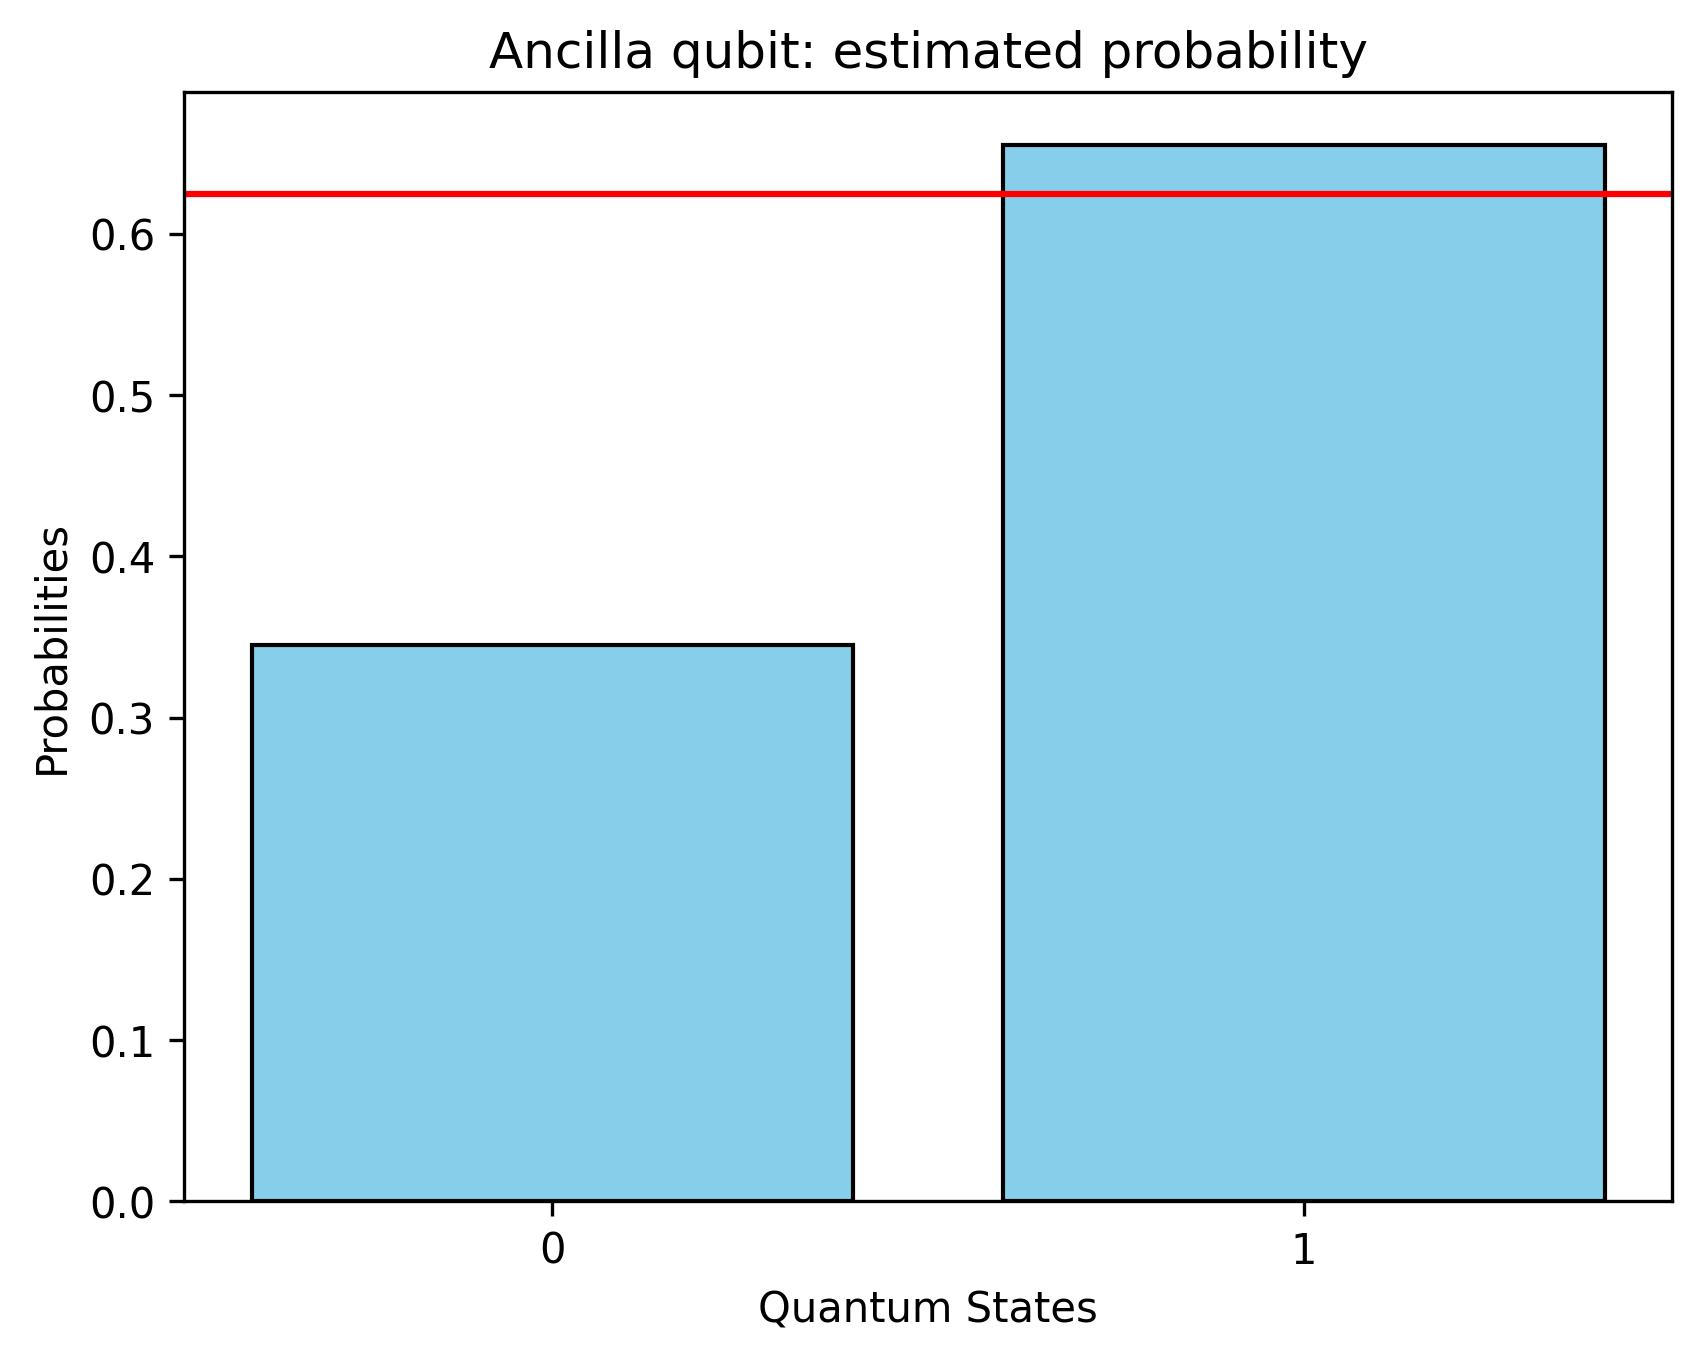
\includegraphics[width=0.75\textwidth]{plots/ibm-prob-anc.jpeg}
    \end{figure}
\end{frame}

\begin{frame}{Simulations: IBM Quantum Hardware}
     \begin{figure}
        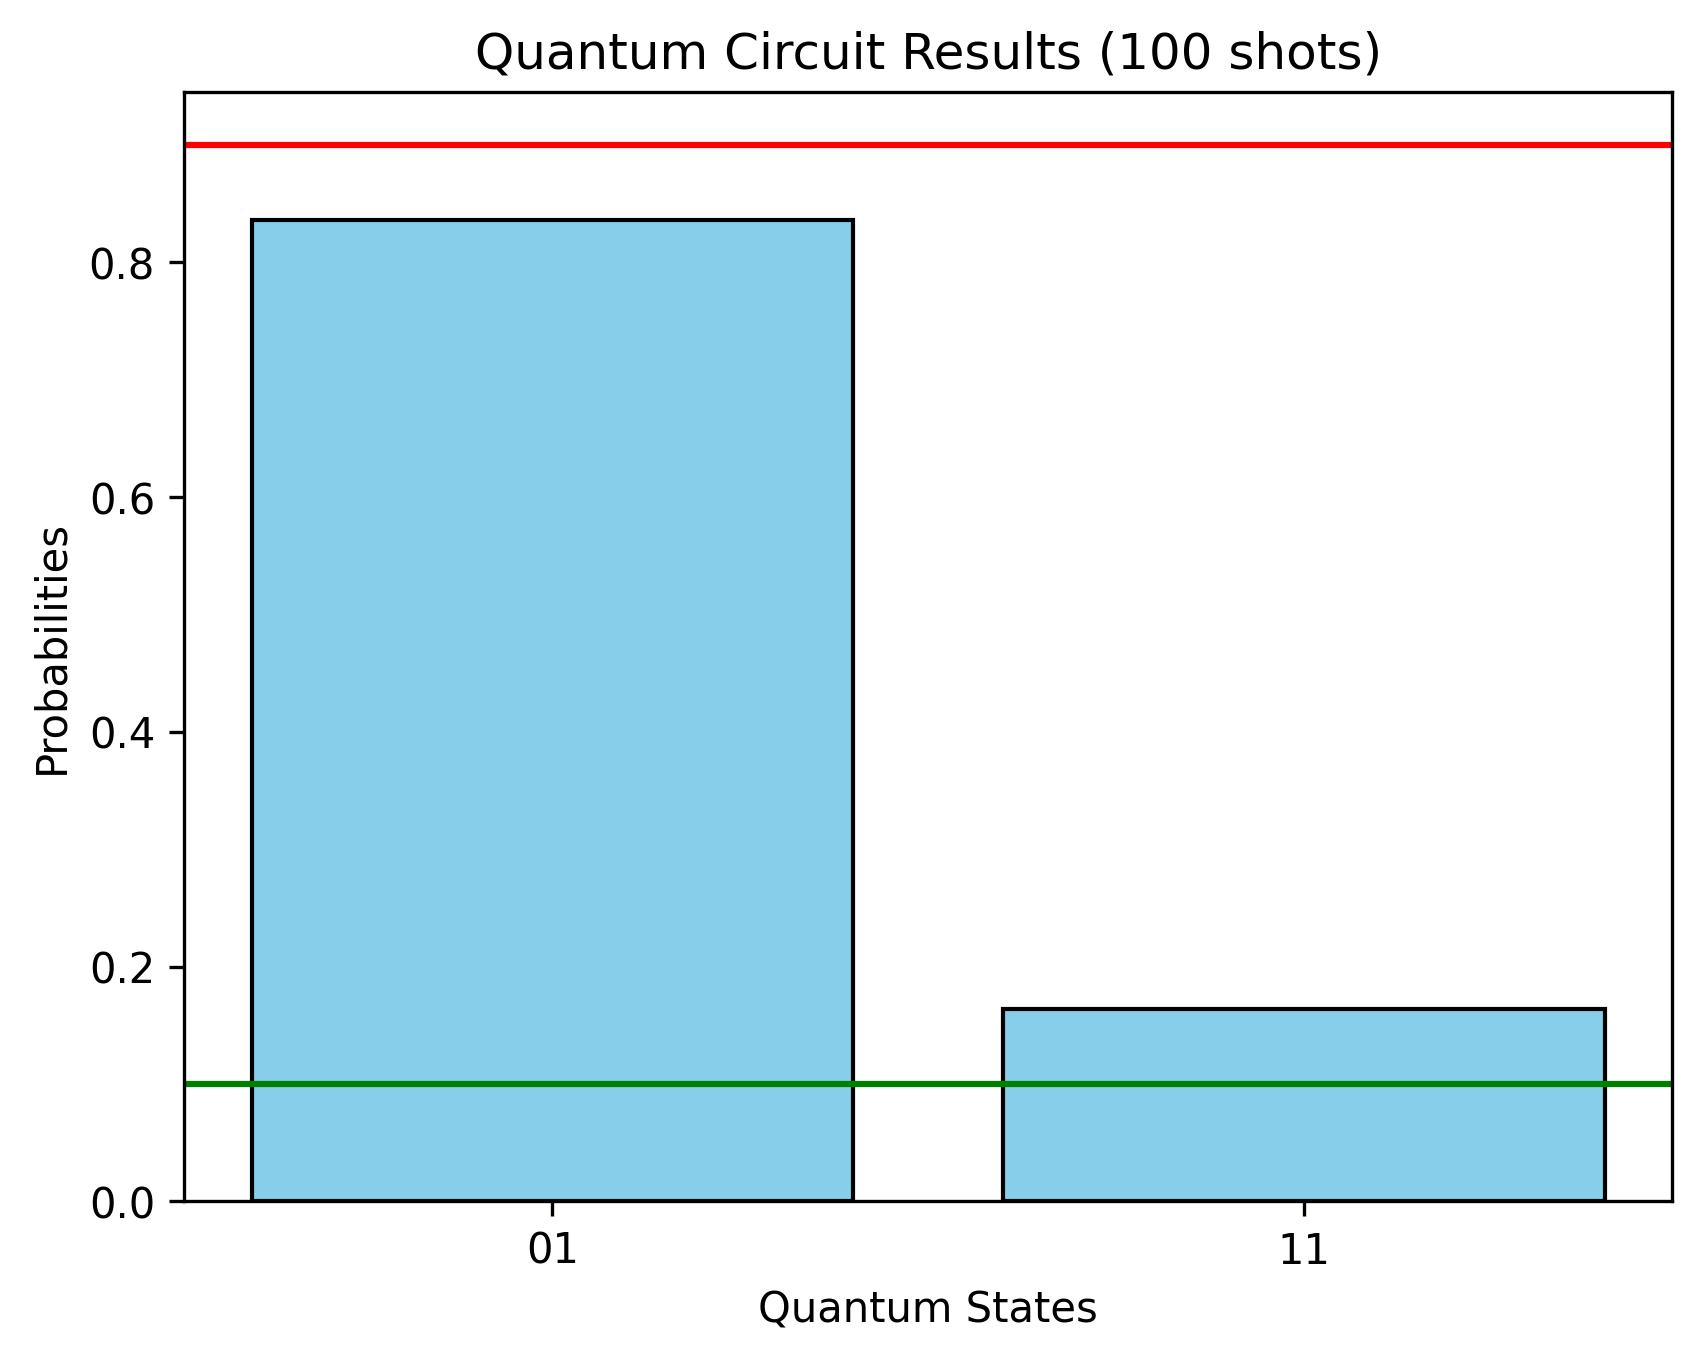
\includegraphics[width=0.75\textwidth]{plots/ibm-conditional-anc1.jpeg}
    \end{figure}
\end{frame}

\begin{frame}{Conclusions}
    
\end{frame}

\begin{frame}{Bibliography}
    \bibliography{references}
\end{frame}